\documentclass[../../main.tex]{subfiles}% 注意这里的文件路径不能用 ./main.tex ,否则用latexmk编译子文件会报错
\graphicspath{{\subfix{./image/}}} % 指定图片目录,后续可以直接使用图片文件名
% 注意这里的文件路径不能用 ../../image/ ,否则用latexmk编译子文件会报错

% 例如:
% \begin{figure}[H]
% \centering
% \includegraphics[scale=0.3]{图.png}
% \caption{}
% \label{figure:图}
% \end{figure}
% 注意:上述\label{}一定要放在\caption{}之后,否则引用图片序号会只会显示??.

\begin{document}

\section{点群}

\begin{definition}
以$O(3)$表示三维Euclid空间的正交变换群.

而以$SO(3)$表示三维Euclid空间的特殊正交变换群,即行列式为1的正交变换构成的群.
\end{definition}
\begin{remark}
显然$SO(3)$中元素都是绕原点的转动,而$O(3)$除转动外,还有镜面反射.
\end{remark}

\begin{proposition}\label{proposition:SO(3)是O(3)的正规子群且商群阶为2}
$SO(3) \lhd O(3)$, $\quad [O(3):SO(3)]=2.$
\end{proposition}
\begin{proof}
由线性代数理论易知.

\end{proof}

\begin{definition}
$O(3)$的有限子群$G$称为\textbf{点群}.

如果点群$G$满足$G \subseteq SO(3)$,则称为\textbf{第一类点群},否则称为\textbf{第二类点群}.
\end{definition}

\begin{theorem}\label{theorem:抽象代数--定理4.9.1}
设$G$是一个第二类点群.令$I=-I_3,$其中$I_3$为三阶单位阵,则有以下结果:
\begin{enumerate}[(1)]
\item $G \cap SO(3)=K$是$G$的正规子群且$[G:K]=2$;

\item 若$I \in G$,则有$G$内直积分解$G=K \otimes \langle I \rangle$;

\item 若$I \notin G$,令$K^+=\{Ig\mid g \in G\setminus K\}$,则$G^+=K \cup K^+$是第一类点群且$G \cong G^+$.
\end{enumerate}
\end{theorem}
\begin{proof}
\begin{enumerate}[(1)]
\item 由\refpro{proposition:SO(3)是O(3)的正规子群且商群阶为2}知$SO(3) \lhd O(3)$,故$\forall g \in K, h \in G$有$hgh^{-1} \in SO(3)$,即有
\begin{align*}
hgh^{-1} \in G \cap SO(3)=K.
\end{align*}
这说明$K \lhd G$,又$g_1, g_2 \in G \setminus K$,则由
\begin{align*}
\det(g_1g_2^{-1})=\det(g_1)\det(g_2^{-1})=(-1)\cdot(-1)=1\Longrightarrow g_1g_2^{-1}\in K
\end{align*}
知$g_1K=g_2K$,因此任取$g'\in G\setminus K,$则$g'K=g''K,\forall g''\in G\setminus K.$而$gK=K,\forall g\in K$.
\begin{align*}
G/K=\{gK\mid g\in G=K\cup (G\setminus K)\}=\{K,g'K\}.
\end{align*}
故$[G:K]=2$.

\item 若$I \in G$,则对$\forall A\in G\setminus K$,有$\det A=-1$,从而$\det \left( IA \right) =1$且$IA\in G$,故$IA\in K$,因此存在$A'\in K$,使得
\begin{align*}
IA=A'\Longrightarrow A=IA'\in IK.
\end{align*}
故$G\setminus K\subseteq IK$.对$\forall IB\in IK$,有$\det \left( IB \right) =-1$,故$IB\notin K$,但$IB\in G$,故$IB\in G\setminus K$,因此$IK\subseteq G\setminus K$.综上$IK=G\setminus K$.于是
\begin{align*}
G=K\cup \left( G\backslash K \right) =K\cup IK=(-IK)\cup (IK)=\{-Ik,Ik\mid k\in K\}=K\{I,-I\}.
\end{align*}
又$\langle I \rangle=\{I,-I\}$为二阶群且$K\cap \langle I \rangle=\{-I\}$.由$(\pm I)g=g(\pm I)(\forall g \in G)$知$\langle I \rangle\lhd G$.故
\begin{align*}
G=K \otimes \langle I \rangle.
\end{align*}

\item 若$I \notin G$,由于$g \in G \setminus K$,故$Ig \in SO(3)$,即
\begin{align*}
G^+=K \cup K^+ \subseteq SO(3).
\end{align*}
令
\begin{align*}
\varepsilon(g)=\frac{1}{2}(1-\det g)=
\begin{cases}
0, & g \in K, \\
1, & g \in G \setminus K.
\end{cases}
\end{align*}
再作$G$到$G^+$的映射$\sigma$如下:
\begin{align*}
\sigma(g)=I^{\varepsilon(g)}g,\ g \in G.
\end{align*}
显然$\sigma$是$G$到$G^+$上的双射,而且对$\forall g_1,g_2\in G$,注意到$I^2=I^0$,故
\begin{align*}
\varepsilon(g_1)+\varepsilon(g_2) = 1-\frac{\det g_1+\det g_2}{2}=\begin{cases}
0, & g_1g_2 \in K, \\
1, & g_1g_2 \in G \setminus K
\end{cases}=\varepsilon(g_1g_2).
\end{align*}
从而
\begin{align*}
\sigma(g_1)\sigma(g_2)&=I^{\varepsilon(g_1)}g_1I^{\varepsilon(g_2)}g_2=I^{\varepsilon(g_1)+\varepsilon(g_2)}g_1g_2 \\
&=I^{\varepsilon(g_1g_2)}g_1g_2=\sigma(g_1g_2)\in G^+,
\end{align*}
即$\sigma$保持乘法且$G^+$对乘法封闭.又因为
\begin{align*}
\sigma \left( g_1 \right) ^{-1}=\left( I^{\varepsilon \left( g_1 \right)}g_1 \right) ^{-1}=I^{\varepsilon \left( g_1 \right)}g_{1}^{-1}=\sigma \left( g_{1}^{-1} \right) \in G^+.
\end{align*}
所以$G^+$对逆元封闭.因此$G^+$为群.故$\sigma$是$G$到$G^+$上的群同构,即$G \cong G^+$.
\end{enumerate}

\end{proof}

\begin{definition}
三维Euclid空间可视为$\mathbf{R}^3$, $x=(x_1,x_2,x_3) \in \mathbf{R}^3$, $x$的长度为
\begin{align*}
|x|=\sqrt{x_1^2+x_2^2+x_3^2}.
\end{align*}
设$r \in \mathbf{R}$且$r>0$,则$S_r=\{x \in \mathbf{R}^3\mid |x|=r\}$为半径为$r$的球面.
\end{definition}
\begin{remark}
显然$\forall g \in O(3), x \in S_r$有$gx \in S_r$.
\end{remark}

\begin{definition}
设$G$为第一类点群,若$x \in S_r$有$g \in G, g \neq \text{id}$,使得
\begin{align*}
gx=x,
\end{align*}
称$x$为$g$的\textbf{极点},也称为$G$的\textbf{极点}.
\end{definition}

\begin{lemma}\label{lemma:抽象代数--引理4.9.1}
设$P$是第一类点群$G$的所有极点的集合,则有以下结果:
\begin{enumerate}[(1)]
\item\label{lemma:抽象代数--引理4.9.1-1} $P$是有限集, $g \in G, g \neq \text{id}$, $g$有且仅有两个极点;

\item\label{lemma:抽象代数--引理4.9.1-2} $\forall g \in G, x \in P$有$gx \in P$,即$G$把极点映为极点.
\end{enumerate}
\end{lemma}
\begin{proof}
\begin{enumerate}[(1)]
\item 若$x$为$g$的极点,即$gx=x$.于是$-x \in S_r, g(-x)=-x$.因此,$-x$亦为$g$的极点.此时$x,-x$是$g$的转动轴与$S_r$的交点,因而对$\forall g \in G, g \neq \text{id}$,$g$有且仅有两点极点,故$P$是有限集.

\item 设$x$是$g_1$的极点, $g \in G$,由
\begin{align*}
(gg_1g^{-1})(gx)=gx
\end{align*}
知$gx$是$gg_1g^{-1}$的极点.
\end{enumerate}

\end{proof}

\begin{corollary}\label{corollary:点群在极点集上的作用--轨道分解和迷向子群}
由\rreflem{lemma:抽象代数--引理4.9.1}{lemma:抽象代数--引理4.9.1-2}知$G$把极点映为极点,故可视$G$作用于极点集$P$上,因而由\rrefthe{theorem:抽象代数--定理4.2.2}{theorem:抽象代数--定理4.2.2-1}知$P$在$G$作用下分成一些$G$的轨道,
\begin{align*}
P=P_1\cup P_2\cup\cdots\cup P_k,\ i\neq j,\ P_i\cap P_j=\varnothing.
\end{align*}
设$x$是一个极点,$G_x=\{g\in G\mid gx=x\}$是$x$的迷向子群,则$|G_x|\geqslant 2$,并且
\begin{align*}
G_{gx}=gG_xg^{-1},\ g\in G.
\end{align*}
若$x\in P_i$,$P_i=\{gx\mid g\in G\}$,则由\refcor{corollary:有限群轨道的阶与其商掉迷向子群的阶相同}知$|P_i|=[G:G_x]$.
\end{corollary}
\begin{proof}
由极点定义知,必存在$g_x\in G\setminus \{\text{id}\}$,使$g_xx=x$.从而$G_x\supseteq \{\text{id},g_x\}$,故$|G_x|\geqslant 2$.

又由\rrefthe{theorem:伴随作用下ad的定义}{theorem:伴随作用下ad的定义-1}知
\begin{align*}
G_{gx}=gG_xg^{-1},\ g\in G.
\end{align*}

\end{proof}

\begin{theorem}
第一类点群$G$的极点集$P$只能分成两个或三个轨道.
\end{theorem}
\begin{proof}
根据\refcor{corollary:点群在极点集上的作用--轨道分解和迷向子群},可设极点集可分解成$k$个轨道,
\begin{align*}
P=P_1\cup P_2\cup\cdots\cup P_k,\ x_i\in P_i.
\end{align*}
又设$|G|=n,\ n_i=|G_{x_i}|,p_i=|P_i|$,其中$G_{x_i}$是$x_i$的迷向子群.于是由\refcor{corollary:点群在极点集上的作用--轨道分解和迷向子群}和\refcor{corollary:抽象代数-推论 1.3.5}知
\begin{align*}
p_i=|P_i|=[G:G_{x_i}]=\frac{n}{n_i},\quad n_i\geqslant 2.
\end{align*}
于是$G_{x_i}$中非恒等元数为$n_i-1=\frac{n}{p_i}-1$.于是对于第$i$个轨道,$G$中以$P_i$中某点为极点的非恒等元的变换数目为
\begin{align*}
\sum\limits_{x\in P_i}|G_x\setminus\{\text{id}\}|=p_i(n_i-1)=n-p_i.
\end{align*}
将每个轨道并起来得到
\begin{align*}
\sum_{x\in P}{|G_x\setminus \{\mathrm{id}\}|}=\sum\limits_{i=1}^k p_i(n_i-1)=\sum\limits_{i=1}^k(n-p_i).
\end{align*}
但注意$G$中除恒等变换外有$n-1$个变换,并且除恒等变换外的每个变换$g$都有两个极点,即若$gx=x$,则$g\in G_x\cap G_{-x}$,故上述计数中每个$g$都重复计数了一次.因而有
\begin{align*}
\sum\limits_{i=1}^k p_i(n_i-1)=2(n-1).
\end{align*}
以$n$除两边,则有
\begin{align}
\sum\limits_{i=1}^k\left(1-\frac{1}{n_i}\right)=2\left(1-\frac{1}{n}\right),\label{eq::::fj38fj90ive90fj9dejkg90w2-3fu90eiu0t4wdszg4.9.1}
\end{align}
其中
\begin{align*}
n\geqslant n_i\geqslant 2.
\end{align*}

若$k=1$,则由式\eqref{eq::::fj38fj90ive90fj9dejkg90w2-3fu90eiu0t4wdszg4.9.1}知$n_1=n$,于是$1-\frac{1}{n}=2\left(1-\frac{1}{n}\right)$,矛盾.

若$k\geqslant 4$,则由式\eqref{eq::::fj38fj90ive90fj9dejkg90w2-3fu90eiu0t4wdszg4.9.1}知
\begin{align*}
\sum\limits_{i=1}^k\left(1-\frac{1}{n_i}\right)=k-\sum\limits_{i=1}^k\frac{1}{n_i}\geqslant k-\frac{k}{2}=\frac{k}{2}\geqslant 2,
\end{align*}
但是$2\left(1-\frac{1}{n}\right)<2$,这就导出矛盾,故$k=2$或$k=3$.


\end{proof}

\begin{theorem}
如果第一类点群$G$的极点分成两个轨道,则$G$只有两个极点$x,-x$.此时$G_x=G_{-x}=G$为$n$阶循环群.
\end{theorem}
\begin{remark}
对于群$G$,有一个简单的几何解释.可以把$g$看成在平面直角坐标系中绕原点旋转$2\pi/n$角,即有
\begin{align*}
g=\begin{pmatrix}
\cos\frac{2\pi}{n}&-\sin\frac{2\pi}{n}\\
\sin\frac{2\pi}{n}&\cos\frac{2\pi}{n}
\end{pmatrix}.
\end{align*}
\end{remark}
\begin{proof}
设$G$的极点集$P$可分解为如下两个轨道:
\begin{align*}
P=P_1\cup P_2,\,x_i\in P_i.
\end{align*}
其中$p_1=|P_1|\geqslant1,p_2=|P_2|\geqslant1$.又设$|G|=n,\ n_i=|G_{x_i}|$,$G_{x_i}$是$x_i$的迷向子群.
由式\eqref{eq::::fj38fj90ive90fj9dejkg90w2-3fu90eiu0t4wdszg4.9.1}有
\begin{align*}
2(1-n^{-1})=1-n_1^{-1}+1-n_2^{-1},\\
\frac{2}{n}=\frac{1}{n_1}+\frac{1}{n_2}=\frac{p_1}{n}+\frac{p_2}{n},
\end{align*}
因此
\begin{align*}
p_1=p_2=1,\ n_1=n_2=n,
\end{align*}
故$G$只有两个极点$x,-x$,因而$G$中每个元素转动轴都是通过$x$与$-x$的直线.设$G$中$n$个元素$\text{id},g_1,\cdots,g_{n-1}$的旋转角分别为
\begin{align*}
0<\theta_1<\theta_2<\cdots<\theta_{n-1}(<2\pi).
\end{align*}
由带余除法,对$i\geqslant 2$有$m_i\in\mathbb{N}$,使得
\begin{align*}
\theta_i=m_i\theta_1+\phi_i,\ 0\leqslant\phi_i<\theta_1.
\end{align*}
于是$g_ig_1^{-m_i}\in G$的旋转角为$\theta_i-m_i\theta_i=\phi_i$.若$\phi_i\neq 0$,则$g_ig_1^{-m_i}$的旋转角与$G$中所有元素都不同,即$g_ig_1^{-m_i}\notin G$矛盾!故$\phi_i=0$,即$g_i=g_1^{m_i}$,从而$G$为循环群且$\theta_1=\frac{2\pi}{n}$.

\end{proof}

\begin{theorem}\label{theorem:抽象代数--定理4.9.4}
如果第一类点群$G$的极点分成三个轨道,在方程\eqref{eq::::fj38fj90ive90fj9dejkg90w2-3fu90eiu0t4wdszg4.9.1}中,设$n_1\leqslant n_2\leqslant n_3$,则有以下情形:
\begin{enumerate}[(1)]
\item $n_1=n_2=2,\ n_3=\frac{n}{2},\ n$为偶数,$n\geqslant 4$;

\item $n_1=2,\ n_2=n_3=3,\ n=12$;

\item $n_1=2,\ n_2=3,\ n_3=4,\ n=24$;

\item $n_1=2,\ n_2=3,\ n_3=5,\ n=60$.
\end{enumerate}
\end{theorem}
\begin{proof}
设$G$的极点集$P$可分解为如下三个轨道:
\begin{align*}
P=P_1\cup P_2\cup P_3,\,x_i\in P_i,\,i=1,2,3.
\end{align*}
其中$p_i=|P_i|\geqslant1.$又设$|G|=n,\ n_i=|G_{x_i}|$,$G_{x_i}$是$x_i$的迷向子群.
方程\eqref{eq::::fj38fj90ive90fj9dejkg90w2-3fu90eiu0t4wdszg4.9.1}可化简为
\begin{align*}
1+\frac{2}{n}=\frac{1}{n_1}+\frac{1}{n_2}+\frac{1}{n_3},\ n\geqslant n_i\geqslant 2.
\end{align*}
由$n_1\leqslant n_2\leqslant n_3$,故$n_1\geqslant 3$时无解.于是有
\begin{align*}
n_1=2,
\end{align*}
此时有
\begin{align*}
1+\frac{2}{n}=\frac{1}{2}+\frac{1}{n_2}+\frac{1}{n_3}.
\end{align*}
若$n_2\geqslant 4$,此时有
\begin{align*}
\frac{1}{2}+\frac{1}{n_2}+\frac{1}{n_3}\leqslant\frac{1}{2}+\frac{1}{4}+\frac{1}{4}=1<1+\frac{2}{n},
\end{align*}
矛盾.故$n_2\geqslant 4$方程时无解.因此$2\leqslant n_2\leqslant3$,即$n_2=2\text{或}3$.
\begin{enumerate}[(1)]
\item 当$n_1=n_2=2$时,此时有
\begin{align*}
\frac{1}{n_3}=\frac{2}{n},
\end{align*}
即$n=2n_3$为偶数.由$n_3\geqslant 2$,故$n\geqslant 4$.

\item 当$n_1=2,\ n_2=3$时有
\begin{align*}
1+\frac{2}{n}=\frac{1}{2}+\frac{1}{3}+\frac{1}{n_3},
\end{align*}
再结合$n>n_1+n_2=5$可得
\begin{align*}
\frac{1}{6}+\frac{2}{n}=\frac{1}{n_3}\Longrightarrow n_3=6-\frac{72}{n+12}\in ( 6-\frac{72}{5+12},6),
\end{align*}
再结合$n_3\geqslant n_2=3$可得
\begin{align*}
3\leqslant n_3\leqslant 5.
\end{align*}
\begin{enumerate}[(i)]
\item 当$n_1=2,\ n_2=3,\ n_3=3$时有$n=12$.

\item 当$n_1=2,\ n_2=3,\ n_3=4$时有$n=24$.

\item 当$n_1=2,\ n_2=3,\ n_3=5$时有$n=60$.
\end{enumerate}
\end{enumerate}


\end{proof}


设第一类点群$G$的极点集$P$分解为如下三个轨道:
\begin{align*}
P=P_1\cup P_2\cup P_3,\,x_i\in P_i,\,i=1,2,3.
\end{align*}
其中$p_i=|P_i|\geqslant1.$又设$|G|=n,\ n_i=|G_{x_i}|$,$G_{x_i}$是$x_i$的迷向子群.由\refthe{theorem:抽象代数--定理4.9.4}知$n_1,n_2,n_3$的取值只有四种情况.
\begin{enumerate}[(1)]
\item 当$n_1=n_2,\ n=2n_3$时,$G$称为\textbf{二面体群},记为$D_{n_3}$.设$T$是平面上一个正$n_3$边形,以$T$的中心$O$为原点,通过$O$垂直$T$的平面的直线为$Oz$轴.$r$为绕$Oz$旋转$\frac{2\pi}{n}$角.显然$r$使正$n_3$边形不变,$r^k(k=0,1,\cdots,n_3-1)$也使正$n_3$边形不变.$T$有$n_3$条对称轴,绕对称轴旋转$180^\circ$也保持$T$不变.所有保持$T$不变的空间转动构成的群就是$G$,极点集$P$为这些转动轴与$S_r$的交点,在$G$的作用下分为三个轨道.

\item 当$n_1=2,\ n_2=3,\ n_3=3,\ n=12$时,群$G$称为\textbf{正四面体群}(tetrahedral group),记为$T$.设$T$为正四面体,以一个顶点与中心的连线为轴旋转$120^\circ,240^\circ$都使$T$不变.以中心与一边的中点的连线为轴旋转$180^\circ$也使$T$不变.所有保持$T$不变的空间转动构成的群就是$G$,极点集$P$为这些转动轴与$S_r$的交点,在$G$的作用下分为三个轨道.

一个正四面体是由4个正三角形围成的多面体.取它的中心为坐标原点,并使其4个顶点的坐标为
\begin{align*}
A_1(-1,-1,1),\ A_2(1,1,1),\ A_3(1,-1,-1),\ A_4(-1,1,-1),
\end{align*}
如\reffig{figure:抽象代数--图4.9.1}所示.
\begin{figure}[H]
\centering
\includegraphics[scale=0.45]{抽象代数--图4.9.1.png}
\caption{}
\label{figure:抽象代数--图4.9.1}
\end{figure}
以$T$表示空间正四面体群,这是使正四面体不变的旋转构成的群.

现在来看看$T$的元素.首先,保持$A_1$不动的变换,除单位变换外,还有绕过$A_1$与$\triangle A_2A_3A_4$中心的直线旋转$120^\circ$与$240^\circ$. 这两个变换有对称群的表示法:$(A_2,A_3,A_4)$与$(A_2,A_4,A_3)$.

同样,可以求出保持$A_2,A_3,A_4$的变换的对称群的表示法
\begin{align*}
(A_1,A_3,A_4),\ (A_1,A_4,A_3),\ (A_1,A_2,A_4),\ (A_1,A_4,A_2),\ (A_1,A_2,A_3),\ (A_1,A_3,A_2).
\end{align*}

此外,绕三个坐标轴旋转$180^\circ$也使正四面体不变,这样又有三个元素,它们的对称群的表示法为
\begin{align*}
(A_2,A_3)(A_1,A_4),\ (A_1,A_3)(A_2,A_4),\ (A_1,A_2)(A_3,A_4).
\end{align*}

不难看出$|T|=12$,而且与4个文字的交错群$A_4$同构.

\item 当$n_1=2,\ n_2=3,\ n_3=4,\ n=24$时,群$G$称为\textbf{正八面体群}(octahedral group),记为$O$.设$T$为正八面体,以一个顶点与中心的连线为轴旋转$90^\circ,180^\circ,270^\circ$都使$T$不变.以中心与一边的中点的连线为轴旋转$180^\circ$也使$T$不变.以中心与一个面的中心的连线为轴旋转$120^\circ,240^\circ$也使$T$不变.所有保持$T$不变的空间转动构成的群就是$G$,极点集$P$为这些转动轴与$S_r$的交点,在$G$的作用下分为三个轨道.

一个正八面体是由8个正三角形围成的多面体.取正八面体的中心为坐标原点,并使正八面体的6个顶点坐标为
\begin{align*}
(\pm1,0,0),\ (0,\pm1,0),\ (0,0,\pm1),
\end{align*}
如\reffig{figure:抽象代数--图4.9.2}所示.
\begin{figure}[H]
\centering
\includegraphics[scale=0.45]{抽象代数--图4.9.2.png}
\caption{}
\label{figure:抽象代数--图4.9.2}
\end{figure}
显然
\begin{align*}
x=\pm1,\ y=\pm1,\ z=\pm1
\end{align*}
这6个平面围成一个立方体.此立方体6个面的中心恰为正八面体的6个顶点,称为正八面体的外接立方体,而
\begin{align*}
x=\pm\frac{1}{2},\ y=\pm\frac{1}{2},\ z=\pm\frac{1}{2}
\end{align*}
这6个面围成一个立方体,它的8个顶点恰好是正八面体8条棱的中点,称为正八面体的内接立方体.

所谓正八面体群$O$即保持正八面体不变的旋转构成的群.由于正八面体与立方体的关系,因而$O$也是使立方体不变的旋转构成的群.

上面正八面体外接立方体的8个顶点的坐标为$(\pm1,\pm1,\pm1)$.记通过点$(1,1,1),(-1,1,1),(-1,-1,1)$与$(1,-1,1)$的4条对角线为$\alpha_1,\alpha_2,\alpha_3$与$\alpha_4$.

显然,$O$中任一元素引起$\alpha_1,\alpha_2,\alpha_3$与$\alpha_4$的一个置换.由于立方体的位置完全由这4条对角线决定,故$O$中不同元素引起$\alpha_1,\alpha_2,\alpha_3$与$\alpha_4$的不同置换.因此,可视$O\subseteq S_4$.另一方面,$S_4$可由$(12),(143)$两个元素生成.事实上记$x=(12),y=(143)$.于是
\begin{gather*}
xyx^{-1}=(243),\ yxy^{-1}=(24),\\
(243)x(243)^{-1}=(14),\ (243)^2x(243)^{-2}=(13).
\end{gather*}
由此可知$(12),(143)$生成$S_4$.
\begin{figure}[H]
\centering
\includegraphics[scale=0.3]{抽象代数--图4.9.3.png}
\caption{}
\label{figure:抽象代数--图4.9.3}
\end{figure}
如\reffig{figure:抽象代数--图4.9.3}所示.通过$A_1A_2$的中点与$S_1'A_2'$的中点的轴在$\square A_1A_2A_1'A_2'$所在的平面内,与$\square A_4A_3A_4'A_3'$垂直且过其中心.绕此轴旋转$180^\circ$,则有$A_3\rightarrow A_3',A_4\rightarrow A_4',A_1\rightarrow A_2,A_1'\rightarrow A_2'$,因而恰好对应变换$(\alpha_1\alpha_2)$.同样能求出其他变换,因而$O\cong S_4$,故以$S_4$代替$O$.

又对角线$\alpha_1=A_1A_1'$垂直于$\triangle A_2A_4A_3'$,于是绕$\alpha_1$旋转$120^\circ,240^\circ$也使立方体不变,而$120^\circ$的旋转恰为$(\alpha_2\ \alpha_3\ \alpha_4)$.

$O$也是使立方体保持不变的群.

\item 当$n_1=2,\ n_2=3,\ n_3=5,\ n=60$时,群$G$称为\textbf{正二十面体群}(icoshedral group),记为$I$.设$T$是正二十面体,是由20个正三角形组成.通过$T$的中心与棱的中点的连线有15条直线,绕这些直线的每一条线旋转$180^\circ$都保持$T$不变.因此,$I$有15个二阶元.这些直线与$S_r$的交点为$I$的极点,并构成一个轨道$P_1,|P_1|=30$,其中一点的迷向子群的阶$n_1=2$.

通过$T$的中心与各面中心的连线有10条,正好是长对角线所在直线.绕这些直线的每一条线旋转$120^\circ,240^\circ$都保持$T$不变.因此,$I$有20个三阶元.这些直线与$S_r$的交点为$I$的极点,并构成一个轨道$P_2,|P_2|=20$,其中一点的迷向子群的阶$n_2=3$.

通过$T$的中心与各顶点的连线有6条,正好是长对角线所在直线.绕这些直线的每一条线旋转$72^\circ$,$144^\circ$,$216^\circ,$ $288^\circ$都保持$T$不变.因此,$I$有24个5阶元.这些直线与$S_r$的交点为$I$的极点,并构成一个轨道$P_3,|P_3|=12$,其中一点的迷向子群的阶$n_3=5$.

因此,$I$是60阶群,$I$的极点集$P$分成三个轨道,$P=P_1\cup P_2\cup P_3$.保持$T$不变的转动群称为正二十面体群,记为$I$.

以正二十面体的各面的中心为顶点,相邻两面的中心的连线为棱,于是构成一个以12个正五边形为面的正十二面体,称为$T$的内接正十二面体(\reffig{figure:抽象代数--图4.9.4}),$I$也保持内接正十二面体不变.
\begin{figure}[H]
\centering
\includegraphics[scale=0.6]{抽象代数--图4.9.4.png}
\caption{}
\label{figure:抽象代数--图4.9.4}
\end{figure}
\end{enumerate}

\begin{theorem}
$\cos72^\circ=\frac{1}{4}(-1+\sqrt{5}),\sin72^\circ=\frac{1}{4}\sqrt{10+2\sqrt{5}}.$

$\omega=\frac{1}{2}(-1+\sqrt{5})$称为\textbf{黄金分割数}.
\end{theorem}
\begin{proof}
设在$\triangle ABC$中,
\begin{align*}
AB=AC=1,\ \angle A=36^\circ,\ \angle B=\angle C=72^\circ.
\end{align*}
作$\angle B$的平分线交$AC$于$E$.于是
\begin{enumerate}[(1)]
\item $\triangle EAB$为等腰三角形且$AE=EB$.
\item $\triangle BCE$为顶角为$36^\circ$的等腰三角形,$EB=BC$,因此$\triangle ABC \sim \triangle BCE,$
\end{enumerate}
从而
\begin{align*}
AC:AE=AC:BC=BC:EC=AE:(AC-AE).
\end{align*}
由$AC=1$有$BC=AE=\frac{1}{2}(-1+\sqrt{5})$,再由正弦定理即得结论.
\begin{figure}[H]
\centering
\tikzset{every picture/.style={line width=0.75pt}} %set default line width to 0.75pt        
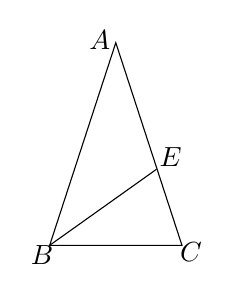
\begin{tikzpicture}[x=0.75pt,y=0.75pt,yscale=-1,xscale=1]
%uncomment if require: \path (0,310); %set diagram left start at 0, and has height of 310

%Shape: Triangle [id:dp9033846557535496] 
\draw   (150.43,47.5) -- (182.3,145.12) -- (118.57,145.12) -- cycle ;
%Straight Lines [id:da5448972142131546] 
\draw    (118.57,145.12) -- (170.01,108.51) ;

% Text Node
\draw (108.24,144) node [anchor=north west][inner sep=0.75pt]    {$B$};
% Text Node
\draw (136.38,40.53) node [anchor=north west][inner sep=0.75pt]    {$A$};
% Text Node
\draw (180.21,142.45) node [anchor=north west][inner sep=0.75pt]    {$C$};
% Text Node
\draw (170.3,96.66) node [anchor=north west][inner sep=0.75pt]    {$E$};
\end{tikzpicture}
\caption{}
\label{figure:黄金分割数证明图}
\end{figure}

\end{proof}

\begin{theorem}
$I$是单群,与$A_5$同构.
\end{theorem}
\begin{proof}
因为$I$的二阶元彼此共轭,构成一个共轭类$C_2$, $c_2=15$;三阶元彼此共轭,构成一个共轭类$C_3$, $c_3=20$;旋转$72^\circ,288^\circ$的元素彼此共轭,构成一个共轭类$C_4$, $c_4=12$;旋转$144^\circ,216^\circ$的元素彼此共轭,构成一个共轭类$C_5$, $c_5=12$.又$C_1=\{\text{id}\}$, $c_1=1$.由此可知$I$是60阶单群.

$I$的Sylow 2子群的个数$2t+1\mid15$,$I$中无4阶元,2的个数为20,因此$2t+1=5$.

设$I$的5个Sylow 2子群为$Y_1,Y_2,Y_3,Y_4$和$Y_5$. $\forall g\in C$,定义$g$在$X=\{Y_1,Y_2,Y_3,Y_4,Y_5\}$上的作用$\Phi(g)$,
\begin{align*}
\Phi(g)Y_i=gY_iG^{-1},\ Y_i\in X.
\end{align*}
于是$\Phi(g)\in S_X\cong S_5$且
\begin{align*}
\Phi(gh)=\Phi(g)\Phi(h),\ \forall g,h\in I.
\end{align*}
因此,$\Phi$是$I$到$S_5$的同态映射,$\Phi(I)$有3阶元与5阶元,因此$\Phi(I)\supseteq A_5$.又因$I$为60阶的单群,故$I\cong A_5$.

\end{proof}



















\end{document}